\documentclass[10pt, oneside]{amsart}
% \usepackage[showboxes]{textpos}

\usepackage[absolute,overlay]{textpos}
	\setlength{\TPHorizModule}{1.0cm}
	\setlength{\TPVertModule}{\TPHorizModule}
	\textblockorigin{0.0cm}{0.0cm}  %start all at upper left corner

\usepackage{amsmath}
\usepackage{amsthm}
\usepackage{amsfonts}
\usepackage{amssymb}
\usepackage{mathpazo}
\usepackage{booktabs}
\usepackage[usenames,x11names]{xcolor}
\usepackage{tikz}
\usepackage{textcomp}
\usepackage[letterpaper]{geometry}
\geometry{verbose,tmargin=0.5in,bmargin=0.5in,lmargin=1in,rmargin=0.5in}
\usepackage{multicol}
\usepackage{bm}
\usepackage{comment}
\usepackage{cancel}
\usepackage{array}
\usepackage{gensymb}
\usepackage{enumerate}

\pagestyle{plain}
\raggedright
\renewcommand{\familydefault}{\sfdefault}
\setlength{\parskip}{\medskipamount}
\setlength{\columnsep}{1cm}

\everymath{\displaystyle}
\setlength{\parskip}{\bigskipamount}

\input{../macros2014}

\begin{document} 






%%%%%%%%%%%%%%%%%%%%%%%%%%%%%%%%%%%%%%%%%%%%%%%%%%%%%%%%%%%%%%%%%%%%%%%%%%%%%%%%%%%%%%%%%%%%%%%%%%%%%%%%%
\begin{textblock*}{1\textwidth}(2cm, 1cm)
	\textbf{Exercise 10}: \\ Nodes $B,\,C,\, D$ and $E$ are all at the same elevation. Given that $y=6.7\,\text{m}$, determine the flow through the system (disregard velocity head at the exit $E$).

	\cfig[0.65]{../Figs/08PipesHW/MT1A}
	
\end{textblock*}

\begin{textblock*}{.35\textwidth}(2cm, 7cm)
	\centering
	
	\begin{tabular}{ccc}
		\toprule
		& Fitting & $Le/D$ \\
		\midrule
		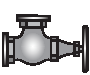
\includegraphics[scale=0.45]{../Figs/08PipesHW/anglevalve} & Angle Valve & 150\\
		\midrule
		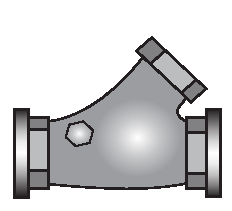
\includegraphics[scale=0.2]{../Figs/08PipesHW/checkvalve} & Check Valve & 100\\
		\midrule
		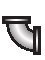
\includegraphics[scale=0.65]{../Figs/08PipesHW/elbow} & Elbow & 50\\
		\midrule
		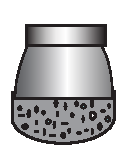
\includegraphics[scale=0.2]{../Figs/08PipesHW/footvalve} & Foot Valve & 75\\
		\midrule
		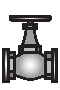
\includegraphics[scale=0.45]{../Figs/08PipesHW/gatevalve} & Gate Valve & 35\\
		\bottomrule
	\end{tabular}
\end{textblock*}


\begin{textblock*}{.35\textwidth}(13cm, 8cm)
	\centering
	
	\begin{tabular}{cccc}
		\toprule
		Pipe & Length (m) & diam (mm) & C\\
		\midrule
		AB & 10 & 500 & 125\\
		\midrule
		BC & 2000 & 275 & 150\\
		\midrule
		BD & 1500 & 250 & 100\\
		\midrule
		DC & 1000 & 300 & 100\\
		\midrule
		CE & 10 & 500 & 125\\
		\bottomrule
	\end{tabular}
\end{textblock*}
%\begin{textblock*}{.6\textwidth}(2cm, 15cm)
	%\cbox{
		%\begin{itemize}
			%\item[] Diam of equiv pipe for BDC (series) = 217.91 mm
			%\item[] Diam of equiv pipe for BC (parallel) = 325.82 mm
			%\item[] Diam of equiv pipe for AE (series) = 324.98 mm
			%\item[] Q = 96.978 L/s
		%\end{itemize}
	%}
%\end{textblock*}
~
\vspace{11cm}

\cmini[0.8]{
	\textbf{Solution}
	\parb
	\cbox{

		The objective is to replace the system of five pipes $AB,\,BC,\,CD,\,DC$ and $CE$ with a single hydraulically equivalent
		pipe from $A$ to $E$. Then we can use the Hazen-Williams equation to find flow through the system.\parb
		Our process will be as follows:
		\begin{enumerate}
			\item Find the effective lengths of the pipes that have valves or fittings.
			\item Consider the series system of two pipes $BD$ and $DC$: find a hydraulically equivalent pipe $BDC$.
			\item Consider the parallel system of two pipes $BDC$ (just found above) and $BC$: find a hydraulically equivalent pipe $BC2$
			for flow from $B$ to $C$.
			\item Consider the series system of three pipes $AB,\,BC2,\text{ and }CE$: find a hydraulically equivalent pipe $AE$.
			\item Use the General Energy Equation and the Hazen-Williams equation to find $Q$.
		\end{enumerate}

	}
}
\parb 
\cmini[0.8]{

	\cbox{
		\textbf{(1)} Find the effective lengths of the pipes that have valves or fittings.

		\begin{align*}
			L_{\text{eff}} &= \text{Actual Length + Diameter}\times\left(\Sigma\frac{L_e}{D}\right) \\\\
			L_{\text{eff}(AB)} &= 10 + 0.5(75+50+100) = 122.5\,\text{m} \\
			L_{\text{eff}(BC)} &= 2000 + 0.275(50+35+50) = 2037.1\,\text{m} \\
			L_{\text{eff}(BD)} &= 1500 + 0.250(150) = 1537.5\,\text{m} \\
		\end{align*}

	}
}
\vfill
\cmini[0.8]{
	\cbox{
		\textbf{(2)} Find a single equivalent pipe $BDC$ for the two pipes $BD$ and $DC$ in series.\parb 

		Find the headloss between $B$ and $C$ for a flow of 100 L/s though $BD$ and $DC$, using the effective lengths of the pipes.

		\begin{align*}
			h_L &= L\left(\frac{279000Q}{CD^{2.63}}\right)^{1.852} \\\\
			h_{L(BD)} &= 1537.5\left(\frac{279000\times 100}{100\times 250^{2.63}}\right)^{1.852} = 39.110\,\text{m} \\
			h_{L(DC)} &= 1000\left(\frac{279000\times 100}{100\times 300^{2.63}}\right)^{1.852} = 10.467\,\text{m} \\\\
			h_{L(BDC)} &= 39.110 + 10.467 = 49.577\,\text{m} \\
		\end{align*}

		\parb 

		Find an equivalent pipe for $BDC$ (i.e., a pipe that has a head loss of 49.577 m for a flow of 100 L/s). We use an equivalent pipe with length 1000 m and resistance coefficient 100, and find the equivalent pipe diameter.

		\begin{align*}
			D_{BDC} &= \left( \frac{279000\times 100}{100\left(\frac{49.577}{1000}\right)^{0.54}}  \right)^{0.3802} = 217.92\,\text{mm}\\
		\end{align*}

	}
}
\parb 
\cmini[0.8]{

	\cbox{
		\textbf{(3)} Now, consider pipe $BC$ and the pipe $BDC$ just found as a parallel system. Find an equivalent pipe for these two parallel pipes.\parb 

		Assume a headloss of 10 m between $B$ and $C$ and find the flow through each of $BC$ and $BDC$:

		\begin{align*}
			Q_{BC} &= \frac{150\times 275^{2.63}\left(\frac{10}{2037.1}\right)^{0.54}}{279000} = 79.262\,\text{L/s}\\
			Q_{BDC} &= \frac{100\times 217.92^{2.63}\left(\frac{10}{1000}\right)^{0.54}}{279000} = 42.084\,\text{L/s}\\
			Q_{BC\text{ and }BDC} &= 79.262 + 42.084 = 121.35 \,\text{L/s}\\
		\end{align*}

		\parb 

		A flow of 121.35 L/s between $B$ and $C$ through both pipes $BC$ and $BDC$ produce a headloss of 10 m. Find an equivalent pipe that replaces these two parallel pipes:

		\begin{align*}
			D_{BC\text{equiv}} &= \left( \frac{279000\times 121.35}{100\left(\frac{10}{1000}\right)^{0.54}}  \right)^{0.3802} = 325.83\,\text{mm}\\
		\end{align*}

	}
	
}
\vfill
\cmini[0.8]{

	\cbox{
		\textbf{(4)} Now we have a series system: $AB,\, BC\text{equiv}$ and $CE$. Assume a flow of 100 L/s from $A$ to $E$, find the total headloss for this flow and then replace these three pipes with a single equivalent pipe.\parb 

		\begin{align*}
			h_{L(AB)} &= 122.5\left(\frac{279000\times 100}{125\times 500^{2.63}}\right)^{1.852} = 0.070450\,\text{m} \\
			h_{L(BC\text{equiv})} &= 1000\left(\frac{279000\times 100}{100\times 325.83^{2.63}}\right)^{1.852} = 7.0000\,\text{m} \\
			h_{L(CE)} &= 10\left(\frac{279000\times 100}{125\times 500^{2.63}}\right)^{1.852} = 0.0057510\,\text{m} \\\\
			h_{L(AE)} &= 0.070450 + 7.0000 + 0.0057510 = 7.0762\,\text{m} \\
		\end{align*}

		\parb 

		Find the equivalent pipe that has a headloss of 7.0762 m for a flow of 100 L/s:

		\begin{align*}
			D_{AE} &= \left( \frac{279000\times 100}{100\left(\frac{7.0762}{1000}\right)^{0.54}}  \right)^{0.3802} = 324.99\,\text{mm}\\
		\end{align*}
	}
	
}
\parb 
\cmini[0.8]{

	\cbox{
		\textbf{(5)} From the General Enery Equation (disregarding velocity head at $E$), headloss through the actual system is 6.7 m. We just need the flow that generates this headloss: \parb 

		\begin{align*}
			Q_{AE} &= \frac{100\times 324.99^{2.63}\left(\frac{6.7}{1000}\right)^{0.54}}{279000} = 96.983\,\text{L/s}\\
		\end{align*}

		
	}
	
}




\end{document}
